\chapter{Foundations of multi-agent reinforcement learning} \label{ch:marl}

\begin{chapter_outline}

This chapter provides a broader overview of reinforcement learning.
We first define reinforcement learning in Section~\ref{sec:ch2_Introduction} and define a stochastic game, a first multi-agent framework, in Section~\ref{sec:ch2_stochastic_Game}.
Multi-agent reinforcement learning is commonly divided into three settings depending on the relative goals of agents as described in Section~\ref{sec:ch2_multi_agent_settings}.
However, a particular setting exists where a single-agent learns, called single-agent reinforcement learning.
In Section~\ref{sec:ch2_single_agent_RL}, we provide essential details on this (\textbf{not so}) particular case where the foundations of multi-agent reinforcement learning approaches lie.
Finally, Section~\ref{sec:ch2_partial_observability} concludes this chapter with a discussion on partial-observability.

\end{chapter_outline}

\section{Introduction} 
\label{sec:ch2_Introduction}
Reinforcement learning is a machine learning setting to solve decision-making problems.
We hereafter paraphrase several reinforcement learning definitions:
\begin{itemize}
\item Reinforcement learning is learning solutions of a sequential decision process by repeatedly interacting with an environment \citep{marl-book}.
%\item Reinforcement learning is a kind of ML where an agent has to learn how to interact with its environment. \citep{pml1Book}.
\item Reinforcement learning is a framework for sequential decision-making, one core topic of ML \citep{introDeepRL}.
\item Reinforcement learning is a method to solve problems where decisions are applied to a system over time to achieve a desired goal \citep{BusoniuErnstBook}.
\item Reinforcement learning is learning by interacting in its environment to maximise a numerical signal called reward \citep{sutton2018reinforcement}.
\end{itemize}

From these definitions, we denote several keywords guiding most RL journeys: environment, interaction, sequence, goal and reward.
But we intentionally left one missing, the agent.
Commonly, an agent is anything capable of acting upon information it perceives from its environment~\citep{russel2010}.
In RL, agent refers to any agent that learns by interacting with its environment, denominated as intelligent or artificial intelligent agents in literature.
Trying to summarise all definitions, we obtain that RL agents interact with their environment by sequentially taking actions that will modify the environment and provide them with a reward, e.g., moving pieces at chess makes the board evolve positions until one wins or draws.
Note that a particular case is a state-less environment not modified by actions, like the bandit problem introduced in Chapter \ref{ch:introduction}.

After defining the agent, we must also consider the number of agents in the environment.
Single-agent reinforcement learning (SARL) becomes multi-agent reinforcement learning (MARL) when more than one agent \textbf{learns}.
We insist on the fact that we consider the number of agents learning.
Indeed, it is possible to have a single learning agent in a multi-agent environment, which can be framed as a single-agent RL problem.
This chapter defines the general multi-agent reinforcement learning framework, followed by three standard settings: cooperation, competition, and general sum.
We then provide an in-depth overview of single-agent reinforcement learning, intending to give enough background to the reader unfamiliar with RL.
We finish with a discussion on partial observability, an essential topic in RL because agents often have uncertainty about their perception of the environment.

Since this chapter aims to provide a broader overview of reinforcement learning and its central concepts, we intentionally skip some details, such as mathematical developments, demonstrations, or definitions.
However, we try to always refer the reader to references to go beyond our introductions.
We acknowledge that the background sections of this manuscript take a lot of inspiration from these cited works, and especially from two of them: ``Reinforcement learning: An introduction'' \citep{sutton2018reinforcement}, well established in the community and ``Multi-Agent Reinforcement Learning: Foundations and Modern Approaches'' \citep{marl-book}, a recent book on the foundations of multi-agent reinforcement learning.
Finally, this manuscript focuses on RL approaches when considering agents interacting in an environment, but other methods exist, and we refer to the book of \cite{russel2010} for many more.

\section{Stochastic game}
\label{sec:ch2_stochastic_Game}

The stochastic game (SG) \citep{stochasticGames} is probably at the foundation of multi-agent reinforcement learning.
In an SG, a set of agents interact with the environment by observing the state of the environment, choosing actions and receiving rewards over a sequence of time, finite or not.
We define a stochastic game by a tuple $[n, \mathcal{S}, \mathcal{U}, R, P, \gamma]$.
The set of agents is $\mathcal{A} \equiv \{1,..,n\}$ so that a specific agent is represented by $a_i$, sometimes directly by $i$, with $i \in \mathcal{A}$.
When not considering a specific one, any agent is represented by $a$.

The interaction of agents in an SG is presented in Figure \ref{fig:ch2_sg}.
At each time step $t$, each agent $a$ selects an action $u_t^a \in \mathcal{U}^a$ based on the state of the environment $s_t \in \mathcal{S}$ with a probability given by its policy $\pi^a(u^a_t|s_t)$, where $\mathcal{S}$ is the state space, and $\mathcal{U}^a$ is the action space of agent $a$.
These $n$ selected actions form the joint action $\mathbf{u} \in \mathcal{U}$, where the joint action space is $\mathcal{U} \equiv \bigtimes_{i \in \mathcal{A}} \mathcal{U}^{a_i}$.
We also denote the joint policy by $\mathbf{\pi}$.
As a consequence of agents taking $\mathbf{u_t}$, the state of the environment $s_t$ transits to a new state $s_{t+1}$ with a probability $P(s_{t+1}, s_t, \mathbf{u_t})$ defined by the stochastic transition function $P:\mathcal{S} \times \mathcal{S} \times \mathcal{U} \rightarrow [0,1]$.

\begin{figure}
    \centering
    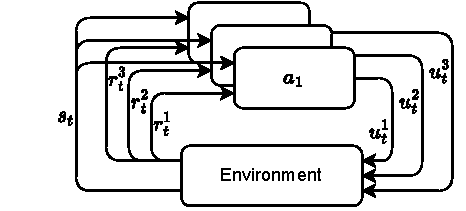
\includegraphics[width=.8\textwidth]{tex_thesis/figures/ch2/SG.pdf}
    \caption{Interaction of agents with the environment in a Stochastic game \citep{stochasticGames}. Agents $i \in \{1,..,n\}$ have access to the state $s_t$ to select actions $u_t^i$. As a consequence, they each receive a reward $r_t^i$ and the environment transitions in a new state $s_{t+1}$.}
    \label{fig:ch2_sg}
\end{figure}

As the state transitions, each agent receives a reward denoted $r_t^{a_i} = R(s_{t+1}, s_t, \mathbf{u_t}, i)$ defined by the reward function $R: \mathcal{S} \times \mathcal{S} \times \mathcal{U} \times \mathcal{A} \rightarrow \mathbb{R}$.
The goal of each agent $a_i$ is to maximise its expected sum of discounted rewards $\mathbb{E}_{\mathbf{\pi}}\left[ \sum_{t=0}^{T-1} \gamma^t r^{a_i}_t \right]$, where $T$ is the time horizon and $\gamma \in ]0, 1]$ the discount factor.
In this thesis, the time horizon $T$ is considered finite, defining the length of an episode.
Intuitively, the discount factor $\gamma$ defines the importance of future reward.
Finally, we insist here that the reward received by an agent depends on the joint action taken and not only on its own.

Several comments can be addressed in the context of the works presented in this manuscript.
In the SG definition, some include an initial state $s_0$ distribution, which we keep implicit (e.g. in \citep{marl-book}).
Since the transition function is stochastic, the reward function is based on the next state obtained, but we sometimes denote it irrespective of this new state for simplicity.
While the state space and action spaces can be composed of discrete or continuous variables, action spaces are discrete in this manuscript.
Agents do not always observe the state of the environment entirely to select an action.
This partial observability is further developed in Section~\ref{sec:ch2_partial_observability}.
Finally, in the literature, an SG is sometimes called a Markov game (e.g. \citep{MarkovGames}).

We cover single-agent reinforcement learning and the corresponding challenges in Section \ref{sec:ch2_single_agent_RL}.
However, many challenges arise in addition to the single-agent ones when multiple agents learn in the environment.
We hereafter highlight the important ones.
As mentioned in the introduction, several settings exist in MARL and addressing these challenges can be easier when considering a specific setting.

The first challenge is the non-stationarity of the learning agents.
Since all agents learn, they all update their strategy over time.
One typical risk is that agents may adapt to the strategy of others in an infinite cycle, as in the rock-paper-scissor example of Chapter \ref{ch:introduction}.
One example solution is finding a Nash equilibrium \citep{nash1950equilibrium}.
Such equilibrium is obtained when no agents are interested in changing their policy, meaning that if one changes its policy, its sum of discounted rewards will decrease.
One problem is that several Nash equilibriums can exist in some environments, and one may provide a better sum of discounted rewards to all agents than another.
This highlights a second challenge in MARL: identifying the optimality of policies.

A third challenge is called credit assignment.
As highlighted in the SG definition, all agents' rewards are based on all agents' actions.
Therefore, each agent must learn whether their action produces a good or bad reward.
This is also a challenge in the single-agent framework, e.g. the agent has to learn to credit actions executed in the past.
Finally, undertaking these three challenges might sound easy with two agents, but it is not.
Moreover, the complexity also scales exponentially with the number of agents.
This is typically the case for the size of joint action space, $|\mathcal{U}|$, and anything that will be a function of it.
These four challenges represent the main challenges in MARL, as presented in \citep{marl-book}.

\section{Multi-agent settings} 
\label{sec:ch2_multi_agent_settings}
The stochastic game definition proposed in Section~\ref{sec:ch2_stochastic_Game} provides a general framework for multi-agent systems.
However, three specific settings are commonly distinguished.
The first setting, cooperation, involves agents cooperating to achieve a common goal.
In the second setting, competition, agents compete to achieve an opposing goal.
The third setting is named general-sum and encompasses everything else.
It is thus convenient to adapt the definition of the stochastic game to these particular settings.

The difference in these settings is the relation between the rewards of agents \citep{marl-book}.
If some agents cooperate, they could have a single reward shared by all agents, or if two agents compete, both can have an equal but opposite reward.
In this Section, we introduce these three settings and identify the two of interest in this manuscript: cooperation and mixed cooperation-competition.
Not much detail will be provided here as these settings are the concern of further chapters.
However, we develop more details about the single-agent setting in the next Section~\ref{sec:ch2_single_agent_RL}.

\subsection{Cooperation} 
\label{sec:ch2_Cooperation}
When agents share the same goal, they cooperate, and it is possible to model with a reward function providing a single reward for all agents instead of a different one per agent.
This is called "common reward games" in \citep{marl-book}.
Many problems can be considered as being a cooperative multi-agent setting.
Examples include robot coordination (e.g. in \citep{papoudakis2021benchmarking}), train scheduling (e.g., in \citep{mohanty2020flatland}), traffic control (e.g. in \citep{zhang2019cityflow}) but also games (e.g., Hanabi \citep{Bard_2020}).
\citet{oroojlooy2022review} provide a review of cooperative MARL, including a more detailed list of applications.

Part~\ref{part:coop} of this manuscript is dedicated to cooperative settings with a common reward.
In Chapter~\ref{ch:cooperation}, we provide the adaptation of the stochastic game definition to a cooperative setting, followed by examples of environments and methods to solve them.
In Chapter~\ref{ch:qvmix}, we present a method to solve such a setting, while in Chapter~\ref{ch:impmarl}, we present a suite of environments which frame a real-world application as a cooperative MARL problem.

\subsection{Competition} 
\label{sec:ch2_Competition}
When agents have opposite goals, they compete.
In competition, any action that benefits one agent incurs a retrofit to other ones.
This setting is also called a zero-sum game \citep{marl-book} because it is often modelled such that the rewards of all agents sum to zero at any time.
In a two-agent zero-sum game, commonly known as a two-player zero-sum game in the game theory literature \citep{russel2010}, a possible adaptation of the stochastic game is to have the reward function providing a single reward.
One agent aims to maximise it while the other tries to minimise it.
We also refer to this setting as fully competitive.
A concrete example is chess with a single reward at the end of the game: $1$ if player 1 won, $0$ if player 1 lost or $1/2$ if players drew.
Player 2's goal would be to minimise this reward, while Player 1 wants to maximise it.
Other examples include card games (e.g. Poker \citep{poker}), board games (e.g. chess, shogi, and Go \citep{silver2018general} or Stratego \citep{stratego}) and video games (e.g. StarCraft II \citep{vinyals2019grandmaster}).


\subsection{General-sum} 
\label{sec:ch2_general_sum}
The third setting includes everything that is not fully cooperative or fully competitive.
Apriori, it is impossible to change the reward function of the general definition as agents' goals are not categorisable.
Maybe one of the best examples of the general-sum setting is autonomous driving \citep{dinneweth2022multi}.

In this manuscript, we are interested in the mixed cooperative-competitive setting where two teams compete against each other.
Examples of this particular setting include games where two teams face each other (e.g., Dota 2 \citep{openai2019dota}).
In this manuscript, we model it with only two reward functions, one per team.
Part~\ref{part:compet} is dedicated to this setting, and we study how methods designed for competition can work alongside cooperation ones.
We provide background in Chapter~\ref{ch:competition}, including necessary background from the competitive literature, and then detail our contribution in Chapter~\ref{ch:2teams}.

\section{Single-agent reinforcement learning} 
\label{sec:ch2_single_agent_RL}
When there is single-agent learning in the environment with RL, it is called single-agent reinforcement learning (SARL).
The most significant part of the history of RL lies in this setting, especially when compared with multi-agent RL.
Indeed, the foundation of MARL relies on many works first proposed in the single-agent framework.
Hence, it serves as our starting point and forms the primary content of this background chapter before diving into MARL.
Specifically, in this Section, we introduce the Markov decision process and discuss some fundamentals of RL that are model-based against model-free, dynamic programming and value-based alongside policy-based methods.

\subsection{Markov decision process}
\label{sec:ch2_mdp}

The definition of a Markov decision process (MDP) can be obtained by considering a single agent in a stochastic game (see Section~\ref{sec:ch2_stochastic_Game}).
We define an MDP as a tuple $[\mathcal{S}, \mathcal{U}, R, P, \gamma, p_0]$ where a single agent interacts with its environment as presented in Figure~\ref{fig:ch2_mdp}.
The agent observes the state $s_t \in \mathcal{S}$ and selects an action from its action space $u_t \in \mathcal{U}$ with a probability defined by its policy $\pi(u_t|s_t)$.
This selected action leads the agent to a new state $s_{t+1}$ with a probability given by the transition function $P:\mathcal{S} \times \mathcal{S} \times \mathcal{U} \rightarrow [0,1]$.
The next state is a function only of the current state and action, called the Markovian property.

\begin{figure}[h]
    \centering
    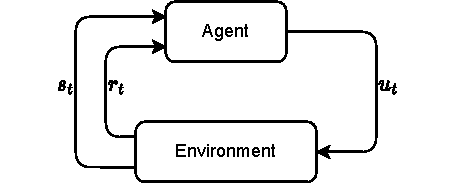
\includegraphics[width=.8\linewidth]{tex_thesis/figures/ch2/MDP.pdf}
    \caption{Interaction of agent with the environment in a Markov decision process \citep{sutton2018reinforcement}. The agent selects one action $u_t$ based on the state $s_t$. As a consequence, it receives a reward $r_t$ and the environment transitions in a new state $s_{t+1}$.}
    \label{fig:ch2_mdp}
\end{figure}

Along the transition of the state, the agent receives a reward $r_t$ defined by the reward function $R:\mathcal{S} \times \mathcal{S} \times \mathcal{U} \rightarrow \mathbb{R}$.
We define the discounted return of a sequence from time step $t$ to time step $T$ as $G_t= \sum_{j=t}^{T-1} \gamma^j r_{t+j}$.
The goal of the agent is to maximise the expected discounted return, so the expected sum of discounted rewards, over a finite episode $\mathbb{E}_{\pi} \left[\sum_{t=0}^{T-1} \gamma^t r_t \right]$, also denoted $\mathbb{E}_{\pi, p_0}\left[ G_0 \right]$ where $p_0$ is the initial distribution of $s_0$.

To achieve maximise its discounted return, the agent needs to learn an optimal policy $\pi^* = \argmax_\pi \mathbb{E}_{\pi}\left[ G_0 \right]$.
To evaluate a policy, we define the state value function $V^\pi(s) = \mathbb{E}_{\pi}\left[G_t|s_t=s\right]$ and the state-action value function $Q^\pi(s, u) = \mathbb{E}_{\pi}\left[G_t|s_t=s, u_t=u\right]$.
While it is meaningless for a single-agent environment, it is interesting to observe that this optimal policy is a Nash equilibrium.
Indeed, the agent can not profit from changing its policy.

Most commonly, two families of methods are identified in RL to learn this optimal policy.
The value-based methods learn a value function and derive the policy from it, while the policy-based methods directly learn a policy.
But before diving into these details, we first discuss whether the model is known or not.

\subsection{Model-based or model-free}
\label{sec:ch2_model_based_vs_model_free}

When solving an MDP, we distinguish methods based on the knowledge of action outcomes.
Indeed, knowing the model of the MDP, one can simulate the environment to evaluate policies \citep{sutton2018reinforcement}.
``A model is a form of reversible access to the MDP dynamics (known or learned)'' \citep{moerland2023model}.
Learning by trial and error without a model is referred to as model-free RL, and this manuscript focuses on methods following this approach.

But when the model is known, two different ways to solve an MDP are distinguished by how they represent the solution.
The historical one is planning, where methods build a local representation of the solution, typically by evaluating solutions around a given state and discarding them after taking action.
It typically does not involve learning anything.
This is how DeepBlue \citep{campbell2002deep} defeated human champions without learning by evaluating many states before taking each action.
The RL approach stores a global solution, typically a policy or a state-action-value function that is learned, whether it has access to the model or not.
This leads to the distinction between model-based RL and planning.
Both have access to the model, but the former uses a global solution while the latter uses local ones.
Knowing the model or learning it is not considered in these definitions of planning and RL, and both exist: learning the model and the solution or learning the model and planning a solution based on it.

This distinction between planning and reinforcement learning does not always agree because, in some methods, a global value function is learned to compute a local representation of the solution, such as in AlphaZero \citep{silver2018general}, considered as model-based RL by some and planning by others.
We finally refer to the work of \cite{moerland2023model} that provides many keys to bridge the gap between RL and planning, between model-based and model-free.
Nevertheless, the following section introduces dynamic programming, a technique requiring a model to compute the optimal policy.
Dynamic programming provides the foundation of model-free methods that are afterwards introduced.

\subsection{Dynamic programming}
Dynamic programming \citep{bellman1966dynamic} methods compute the optimal policy given a model of an MDP \citep{sutton2018reinforcement}.
They rely on the property that the value functions $V^{\pi^*}$ and $Q^{\pi^*}$ of the optimal policy ${\pi^*}$ satisfy the Bellman equations $\forall s, u$:
\begin{equation}
\label{eq:ch2_bellmanV}
    V^{\pi^*}(s) = \max_u \mathbb{E}[r_t + \gamma V^{\pi^*}(s_{t+1})| s_t=s, u_t=u],
\end{equation}
\begin{equation}
\label{eq:ch2_bellmanQ}
    Q^{\pi^*}(s, u) = \mathbb{E}[r_t + \gamma \max_{u'} Q^{\pi^*}(s_{t+1}, u') |s_t=s, u_t=u].
\end{equation}

Not going into the details of policy evaluation, policy improvement, policy iteration and value iteration, e.g. presented in \citep{sutton2018reinforcement}, one can find the optimal policy by iteratively evaluating and improving the policy with the value functions.
This can be highlighted by developing the value functions for any policy $\pi$ and $\forall s, u$:
\begin{equation}
\label{eq:ch2_V_2}
\begin{split}
    V^\pi(s)= \mathbb{E}_{\pi}\left[G_t|s_t=s\right] & = \mathbb{E}_{\pi}\left[r_t + \gamma V^\pi(s_{t+1})|s_t=s\right]\\
     & = \sum_{u} \pi(u|s) \sum_{s'} P(s', s, u) (R(s', s, u) + \gamma V^\pi(s')),
\end{split}
\end{equation}
\begin{equation}
\label{eq:ch2_Q_2}
\begin{split}
    Q^\pi(s, u) = \mathbb{E}_{\pi}\left[G_t|s_t=s, u_t=u\right] & = \mathbb{E}_{\pi}\left[r_t + \gamma V^\pi(s_{t+1})|s_t=s, u_t=u \right] \\
    &  = \sum_{s'} P(s', s, u) (R(s', s, u) + \gamma V^\pi(s')).
\end{split}
\end{equation}

In addition to requiring the model knowledge $P$ and $R$, the complexity of these methods increases with the size of the state space, often referred to as the curse of dimensionality, which may limit their usage.
Because of our direction towards model-free RL, without the model knowledge, our interest here is to present Equations~\ref{eq:ch2_bellmanV},~\ref{eq:ch2_bellmanQ},~\ref{eq:ch2_V_2} and~\ref{eq:ch2_Q_2} that may ease the understanding of further concepts.


\subsection{Value-based methods} \label{sec:ch2_value_based_methods}
Value-based methods are designed to learn value functions.
Maybe one of the first methods in model-free RL is Q-learning \citep{watkins1992q}, where the state-action value function learned is the optimal one defined as $Q^{\pi^*}(s, u)=\max_{\pi}Q^\pi(s, u)$.
This enables the agent to greedily select the action $\pi^*(u|s)=\argmax_u Q^{\pi^*}(s, u)$.

Q-learning is a tabular method because it maintains $Q(s, u)$ estimations in a table, one value for each state-action pair.
It updates these estimations based on themselves, called bootstrapping, and is based on temporal difference (TD) learning.
Following the update 
\begin{equation}
\label{eq:ch2_QLearning}
    Q(s_t, u_t) \leftarrow Q(s_t, u_t) + \alpha \left[ r_t + \gamma \max_u Q(s_{t+1}, u) - Q(s_t, u_t) \right],
\end{equation}
one can repeatedly update the estimation $Q(s, u)$ by adding the temporal difference weighted by a learning rate $\alpha$ controlling the update size.

It is important to denote that this algorithm allows approximating $Q^{\pi^*}(s, u)$ independently of the policy used to sample transitions ($s_t, u_t, r_t, s_{t+1}$).
These transition samples are typically generated with an $\epsilon$-greedy policy that takes a random action instead of the greedy one with a probability $\epsilon$.
This is a characteristic of the off-policy methods, whereas the on-policy methods improve the policy used to generate the transitions.
In this manuscript, we consider only value-based methods that are off-policy, but on-policy methods are discussed further in Section~\ref{sec:ch2_Cooperation}.
To cite one, SARSA is a well-known on-policy value-based method, e.g. in \citep{sutton2018reinforcement}.

Despite being independent of the policy, this iterative process highlights the exploration-exploitation dilemma in RL.
Either you only play the action that maximises your currently learned value function, and therefore, you exploit, or you play a different action and explore the possible outcomes.
Balancing between exploration and exploitation is a key parameter to train agents.

Back to Q-learning, the table size to maintain increases as the state-action space size increases.
Therefore, it can become impractical to compute an estimate of $Q(s, u)$ for each state-action pair, requiring function approximators.
Various function approximators exist, but we restrict ourselves to neural networks in this manuscript.

A neural network is a function $f: \mathcal{X} \rightarrow \mathcal{Y}$ that maps an input ($\in\mathcal{X}$) to an output ($\in\mathcal{Y}$) based on its parameters $\theta$: $y = f(x;\theta)$.
These parameters define a sequence of differentiable functions, linear or not, allowing optimising the parameters by following the gradient of an objective, commonly called a loss function $\mathcal{L}(\theta)$.
To minimise the loss, parameters can be updated by gradient descent: $\theta = \theta - \alpha \nabla \mathcal{L}(\theta)$.
Optimising a neural network is also referred to as training it.
Many loss functions exist to train neural networks, depending on the function to be approximated.
Nowadays, neural networks are very large, leading to the name of deep learning.
We refer to \citep{zhang2023dive} or \citep{prince2023understanding} for many more details.
Finally, reinforcement learning with neural networks is called deep reinforcement learning, e.g. in \citep{introDeepRL}.
As it became common to use neural networks in RL, we decided to remove the word "deep" from the taxonomy, as the title of this manuscript should be "Contributions to deep multi-agent reinforcement learning".
In the following, we introduce how to train such networks to approximate a value function and, in Section~\ref{sec:ch2_policy_based_methods}, to approximate a policy.

A standard method in RL, referred to as deep Q-network (DQN) \citep{Mnih2015}, is to approximate $Q(s, u)$ with a neural network $\theta$.
This can be achieved by minimising the loss 
\begin{equation}
\label{eq:ch2_dqnloss}
    \mathcal{L}(\theta) = \mathbb{E}_{\langle . \rangle\sim B} \big[\big(r_{t} + \gamma \max_u Q(s_{t+1}, u; \theta')- Q(s_{t}, u_{t}; \theta)\big)^{2}\big]
\end{equation}
where $B$ is the replay buffer and $\theta'$ is the target network.
The replay buffer $B$ stores transitions $\langle s_{t},u_{t},r_{t},s_{t+1}\rangle$ from which batches of transitions are sampled to update $\theta$ \citep{lin1992self}.
This replay buffer allows updating the neural network with past transitions.
The target network $\theta'$ is a copy of $\theta$ updated periodically that reduces the moving target problem as $\theta$ is updated several times before updating $\theta'$, e.g., in \citep{Mnih2015}.

In both Equations~\ref{eq:ch2_QLearning} and~\ref{eq:ch2_dqnloss}, the $max$ operator can introduce some positive bias. 
To overcome this bias, a method called Double Q-learning \citep{hasselt2010double}, and adapted to Q-learning with approximations \citep{van2016deep}, consists in selecting the action that maximises the updated $Q(., \theta)$ to compute the target state-action value.
The corresponding loss is 
\begin{equation}
    \label{eq:ch2_doubleQ}
    \mathcal{L}(\theta) = \mathbb{E}_{\langle . \rangle\sim B} \big[\big(r_{t} + \gamma Q(s_{t+1}, \argmax_u Q(s_{t+1}, u;\theta) ; \theta')- Q(s_{t}, u_{t}; \theta)\big)^{2}\big].
\end{equation}

Double Q-learning, also called DDQN, is one of the possible improvements of DQN, and we refer to the Rainbow paper \citep{hessel2018rainbow} that addresses several others.
To cite one, the extension to distributional RL, which approximates distributions instead of expected returns, can be of interest \citep{bellemare2017distributional, THEATE2023199}. 

\subsection{Policy-based methods} \label{sec:ch2_policy_based_methods}
Policy-based methods are designed to learn the policy.
In this manuscript, we restrict to the subclass of policy gradient methods where a neural network parametrised by $\theta$ approximates a differentiable policy $\pi_\theta=\pi(u|s;\theta)$.
Policy gradient methods hence update $\theta$ to find the optimal policy that maximises the expected return denoted as  $J(\pi_\theta) = \mathbb{E}_{\pi_\theta}[G_0]$.
Maybe one of the first method is REINFORCE \citep{williams1992simple} which updates $\theta = \theta + \alpha \nabla_\theta J(\pi_\theta)$ by ascending the gradient
\begin{equation}
\label{eq:ch2_reinforce_grad}
    \nabla_\theta J(\pi_\theta) = \nabla_\theta \mathbb{E}_{\pi_\theta}[G_0] = \mathbb{E}\left[\sum_{t=0}^{T-1} Q(s_t, u_t) \nabla_\theta \log \pi(u_t|s_t;\theta)\right].
\end{equation}

Estimating $Q(s_t, u_t)$ instead of computing it is a solution proposed by the actor-critic methods \citep{sutton1999policy,konda1999actor}.
This type of method expands upon REINFORCE by incorporating a second neural network, called the critic and denoted by $\phi$, that estimates $Q(s_t, u_t;\phi)$ while the actor is the parametrised policy $\pi(u|s;\theta)$.
The new gradient provided by incorporating the critic is
\begin{equation}
\label{eq:ch2_Q_actor_crit}
    \nabla_\theta J(\pi_\theta) = \mathbb{E}\left[\sum_{t=0}^{T-1} Q(s_t, u_t;\phi) \nabla_\theta \log \pi(u_t|s_t;\theta)\right].
\end{equation}

Moreover, a baseline can be injected into the gradient to reduce variance.
Usually, the baseline is  $V(s)$, independent of the action taken, and $Q(s, u;\phi)$ is replaced by the advantage function $A(s,u; \phi)$ \citep{10.5555/2074022.2074088}, leading to

\begin{align}
\begin{split}
\label{eq:ch2_baseline_actor_crit}
    \nabla_\theta J(\pi_\theta)
    & = \mathbb{E}\left[\sum_{t=0}^{T-1} [Q(s_t, u_t) - V(s_t)] \nabla_\theta \log \pi(u_t|s_t;\theta)\right]\\
    & = \mathbb{E} \left[\sum_{t=0}^{T-1} A(s_t, u_t; \phi) \nabla_\theta \pi(s_t, u_t; \theta)\right].
\end{split}
\end{align}

Estimating the advantage with only one neural network is possible either by $A(s_t,u_t; \phi)=Q(s_t, u_t;\phi)-\sum_u \pi(u|s_t;\theta) Q(s_t,u; \phi)$ or by $A(s_t,u_t; \phi)=r_t +\gamma V(s_{t+1};\phi) - V(s_t;\phi)$.
This critic can be trained on-policy or off-policy following methods described in Section~\ref{sec:ch2_value_based_methods}.
This is why actor-critic methods are sometimes described as a mix between value-based and policy-based methods.

Nowadays, advanced policy-based methods relying on the actor-critic paradigm appear to be the most successful.
We can cite trust region policy optimisation (TRPO) \citep{schulman2015trust} and its variant proximal policy optimisation (PPO) \citep{schulman2017ppo}.
Both methods rely on a controlled policy update by constraining the loss of REINFORCE defined in Equation~\ref{eq:ch2_reinforce_grad}.

Finally, there is no epsilon-greedy policy to balance the exploration-exploitation dilemma in policy-based methods.
However, adding a penalizing term in the gradient has been justified to improve exploration.
An example is entropy regularisation \citep{williams1991function}, where we penalize a low entropy of the policy outcomes.
However, \cite{bolland2024behind} has demonstrated that such techniques change the learning objective and increase the chance of updating the policy toward the optimal one, which is different from exploring new actions.

\section{Partial observability} \label{sec:ch2_partial_observability}
As defined in previous sections, the Markov decision process and the stochastic game are fully observable.
Agents have complete access to the state environment and perceive everything without uncertainty.
In real-world applications, it is not always possible to consider this feasible.
Anyone can come up with ideas of a partially observable environment.
Especially given our definition of agents ``acting upon information it perceives''.

Starting with SARL the Markov decision process is said to be a partially observable MDP (POMDP) \citep{KAELBLING199899} when the agent has only access to incomplete information about the state.
The definition of a POMDP is obtained easily from the MDP definition of Section~\ref{sec:ch2_mdp} by adding an observation space $\mathcal{Z}$ and an observation function $O:\mathcal{S} \times \mathcal{Z} \rightarrow [0, 1]$, mapping a state and an observation to the probability of observing the latest.
The corresponding interaction diagram of a POMDP is presented in Figure \ref{fig:ch2_pomdp}.

\begin{figure}
    \centering
    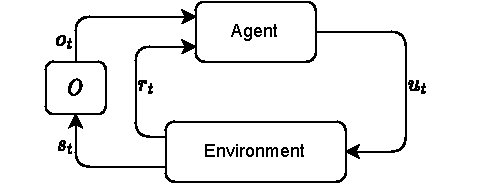
\includegraphics[width=.8\linewidth]{tex_thesis/figures/ch2/POMDP.pdf}
    \caption{Interaction of agent with the environment in a partially observable Markov decision process\citep{KAELBLING199899}. The agent does not have access to the state $s_t$ but to an observation $o_t$ defined by the observation function $O$. Based on $o_t$, it selects one action $u_t$. As a consequence, it receives a reward $r_t$ and the environment transitions in a new state $s_{t+1}$.}
    \label{fig:ch2_pomdp}
\end{figure}

As it cannot fully observe the environment, the agent's policy $\pi$ can no longer be a function of the state.
One solution is to define the policy as a function of the observation.
However, this solution cannot be considered because the observation usually does not respect the Markovian property defined in Section~\ref{sec:ch2_mdp}.
This is why in POMDP, the policy is commonly a function of the history of past observations and actions $\tau=(\mathcal{Z} \times \mathcal{U})^\tau$, in addition to the current observation, denoted $\pi(u_t|\tau_t,o_t): (\mathcal{Z} \times \mathcal{U})^t \rightarrow [0,1]$.
Some authors prefer to include the current observation in $\tau$, allowing them to write $\pi(u_t|\tau_t)$ and, to improve readability, we sometimes do it as well.
The corresponding $Q$ function is typically denoted $Q(\tau,u)$ instead of $Q(\tau, o, u)$.

To solve a POMDP, a solution is to compute the policy based on a belief $b(s)=Pr(s|\tau,o)$, the probability of being in a given state, knowing the history of observations and actions.
However, in practice, the history of an agent can become very large, which can be impractical.
As in the different methods previously defined, the belief can be approximated with recurrent neural networks (RNN), such as GRU \citep{Chung2014EmpiricalModeling} or LSTM \citep{Hochreiter1997LongMemory}.
These networks typically take timeseries as input and maintain a hidden state, updated at each timestep of one timeseries, which can be considered a memory.
Recurrent networks have many applications, and in POMDP, their hidden state allows maintaining a belief without processing the whole history at each timestep.

Using recurrent networks to compute policies is thus a common practice in POMDP, resulting in recurrent policies.
Adding RNN has demonstrated convincing results, such as in recurrent policy gradients \citep{wierstra2010recurrent} or in deep recurrent Q-network (DRQN) \citep{Hausknecht2015DeepMDPs}.
We suggest readers interested in details read the pedagogical paper of \cite{lambrechts2022recurrent}.
This paper demonstrates that the correlation between the hidden state of RNNs, used to approximate policies, and the belief increases as the training progresses.

Adding partial observability in the definition of the stochastic game leads to the most general framework of multi-agent reinforcement learning, the partially observable stochastic game (POSG) \citep{hansen2004dynamic}.
Its definition is obtained by adding a set of $n$ observation spaces $\mathcal{Z}$ and a set of $n$ observation functions $\mathcal{O}$ in the definition of the SG.
A shortcut in this manuscript, and sometimes in the literature, is to consider that these two sets $\mathcal{Z}$ and $\mathcal{O}$ are singleton, the single observation function $O:\mathcal{S} \times \mathcal{A} \rightarrow \mathcal{Z}$ therefore maps an observation from the state and a given agent.

An agent's belief in a POSG should be considered differently from that in a POMDP \citep{DecPomdp}.
Being in a given state is not only a function of one agent's history but is a function of all agents' history.
Even when agents can fully observe the current state, they may not observe the actions previously taken by others.
However, this manuscript does not address multi-agent belief, and we refer to \citep{DecPomdp} for more details.
In a POSG, we consider that an agent's policy is a function $\pi^{a}(u_t^{a}|\tau_t^{a},o_t^{a}): (\mathcal{Z}^a \times \mathcal{U}^a)^t \rightarrow [0,1]$, which maps its history $\tau_t^{a} \in (\mathcal{Z}^a \times \mathcal{U}^a)^{t-1}$ and its current observation $o_t^{a}$ to the probability of taking action $u_t^{a}$.
As in SARL, such a policy is commonly a recurrent policy approximated with RNN.

